%	This LaTeX file is written by Zhiyang Ong as a template for creating presentation slides.

%	The MIT License (MIT)

%	Copyright (c) <2015> <Zhiyang Ong>

%	Permission is hereby granted, free of charge, to any person obtaining a copy of this software and associated documentation files (the "Software"), to deal in the Software without restriction, including without limitation the rights to use, copy, modify, merge, publish, distribute, sublicense, and/or sell copies of the Software, and to permit persons to whom the Software is furnished to do so, subject to the following conditions:

%	The above copyright notice and this permission notice shall be included in all copies or substantial portions of the Software.

%	THE SOFTWARE IS PROVIDED "AS IS", WITHOUT WARRANTY OF ANY KIND, EXPRESS OR IMPLIED, INCLUDING BUT NOT LIMITED TO THE WARRANTIES OF MERCHANTABILITY, FITNESS FOR A PARTICULAR PURPOSE AND NONINFRINGEMENT. IN NO EVENT SHALL THE AUTHORS OR COPYRIGHT HOLDERS BE LIABLE FOR ANY CLAIM, DAMAGES OR OTHER LIABILITY, WHETHER IN AN ACTION OF CONTRACT, TORT OR OTHERWISE, ARISING FROM, OUT OF OR IN CONNECTION WITH THE SOFTWARE OR THE USE OR OTHER DEALINGS IN THE SOFTWARE.

%	Email address: echo "cukj -wb- 23wU4X5M589 TROJANS cqkH wiuz2y 0f Mw Stanford" | awk '{ sub("23wU4X5M589","F.d_c_b. ") sub("Stanford","d0mA1n"); print $5, $2, $8; for (i=1; i<=1; i++) print "6\b"; print $9, $7, $6 }' | sed y/kqcbuHwM62z/gnotrzadqmC/ | tr 'q' ' ' | tr -d [:cntrl:] | tr -d 'ir' | tr y "\n"



%%%%%%%%%%%%%%%%%%%%%%%%%%%%%%%%%%%%%%%%%%%%%%
%	Preamble

%	Acknowledgement:
%		This is based on a template provided to me by Dott. Francesco Stefanni, from the University of Verona in January 2011.
%
%	Number the slides per section. This makes it easier to track the index of the slides (or number of slides) per section, as opposed to the cumulative number of slides. When I manually track the number of slides for a presentation, each time I refactor the set of slides, I would have to update the slide numbers. I want the computer to do this automatically. Hence, I shall not do this manually.



%	Use the Beamer package to create the presentation slides.
\documentclass[xcolor={usenames,dvipsnames},hyperref={hyperindex,bookmarks}]{beamer}


%%%%%%%%%%%%%%%%%%%%%%%%%%%%%%%%%%%%%%%%%%%%%%
%	Import and Customize LaTeX packages.
\usepackage{beamerthemesplit}


%	Package for typesetting the following symbol: $\mathfrak{S}$
%\usepackage{amssymb}

%\mode<presentation>
%{ \usetheme{boxes} }

%	Select the presentation mode.
\mode<presentation>{
	\usetheme[logos=true,pagenumbers=true,background=true]{Esd}
}
\setbeamercovered{transparent}
%\setbeamercovered{invisible}


%	Import package to facilitate typesetting of algorithms.
\usepackage{listings}

\lstset{
  language=C++,
  tabsize=4,
%  basicstyle=\ttfamily\color{black}\small,
  basicstyle=\ttfamily\color{black},
%  backgroundcolor=\color{lightgray},
%  backgroundcolor=\color{white},
  keywordstyle=\color{Purple}\bfseries,
  identifierstyle=\color{OliveGreen},
  commentstyle=\color{Gray}\itshape,
  stringstyle=\color{CarnationPink},
  showstringspaces=false,
  showtabs=false,
  showspaces=false
}


\definecolor{lightgray}{gray}{0.95}
\font\emailtt=cmtt9

%	Set up configuration for hyperlinks.
%\usepackage[pdftex]{hyperref}	-- Option clash
\hypersetup{
    pdftitle={{\it PULPino} attack scenarios},     % title
    pdfauthor={Zhiyang Ong},                 % author
    pdfsubject={Hack@DAC 2018 Contest}, % subject of the document
    pdfcreator={Creator},                           % creator of the document
    pdfproducer={dvipdft},                          % producer of the document
% Modified by Zhiyang Ong on Feb 7, 2011 to improve the way hyperlinks are colored in these presentation slides
	pdfkeywords={LaTeX, graphics, color},
%    pdfkeywords={C, C++, programming style},        % list of keywords
%
%    bookmarks=true,         % show bookmarks bar?
    unicode=false,          % non-Latin characters in Acrobats bookmarks
    pdftoolbar=true,        % show Acrobats toolbar?
    pdfmenubar=true,        % show Acrobats menu?
    pdffitwindow=false,     % window fit to page when opened
% Modified by Zhiyang Ong on Feb 7, 2011 to improve the way hyperlinks are colored in these presentation slides
	pdfpagemode=UseOutlines,bookmarks, bookmarksopen,
	pdfstartview=FitH, colorlinks, linkcolor=blue, citecolor=blue, urlcolor=red,
%    pdfstartview={Fit},    % fits the width of the page to the window
    pdfnewwindow=true,      % links in new window
% Modified by Zhiyang Ong on Feb 7, 2011 to improve the way hyperlinks are colored in these presentation slides
	colorlinks=red,        % false: boxed links; true: colored links
	linkcolor=red,          % color of internal links
%    colorlinks=false,        % false: boxed links; true: colored links
%    linkcolor=red,          % color of internal links
    citecolor=green,        % color of links to bibliography
    filecolor=magenta,      % color of file links
    urlcolor=red,           % color of external links
    pdfpagemode=FullScreen
    %
    %pdfpagelabels=false
}

%\usepackage[all]{hypcap}




%%%%%%%%%%%%%%%%%%%%%%%%%%%%%%%%%%%%%%%%%%%%%%
%	Added by Zhiyang Ong on Feb 7, 2011 to allow figures to be places side-by-side
%\usepackage{subfigure}









%%%%%%%%%%%%%%%%%%%%%%%%%%%%%%%%%%%%%%%%%%%%%%
%%%%%%%%%%%%%%%%%%%%%%%%%%%%%%%%%%%%%%%%%%%%%%
%%%%%%%%%%%%%%%%%%%%%%%%%%%%%%%%%%%%%%%%%%%%%%
%%%%%%%%%%%%%%%%%%%%%%%%%%%%%%%%%%%%%%%%%%%%%%
%%%%%%%%%%%%%%%%%%%%%%%%%%%%%%%%%%%%%%%%%%%%%%
%%%%%%%%%%%%%%%%%%%%%%%%%%%%%%%%%%%%%%%%%%%%%%
%%%%%%%%%%%%%%%%%%%%%%%%%%%%%%%%%%%%%%%%%%%%%%


%	Quantum Model Checking Is Not Evil: It Is Mandatory For Quantum Robots


%	First slide of the presentation
\title[Hack@DAC 2018 Contest]
{\huge 
{\it PULPino} attack scenarios \&\ Defense}
\subtitle{How to hack the {\it PULPino} platform? And, defend it.}
\author{Zhiyang Ong}
\institute{
	Department of Electrical and Computer Engineering \\
	Dwight Look College of Engineering,\\
	Texas A\&M University \\
	College Station, TX
}
\date{\today}	% (optional)
\subject{Subject Title}

%	This set of presentation slides is based on \cite{Ying2014a}, from my BibTeX research database.







%%%%%%%%%%%%%%%%%%%%%%%%%%%%%%%%%%%%%%%%%%%%%%
%	Do nothing in this section of the LaTeX document

\begin{document}

\begin{frame}
\titlepage
\end{frame}



%	Table of Contents
\AtBeginSection[]		% Do nothing for \subsection*
{
	\begin{frame}
%		\frametitle{\textcolor{yellow}{Table of Contents}}
		\frametitle{Table of Contents}
%		\textcolor{yellow}{\tableofcontents[currentsection]}
		\tableofcontents[currentsection,currentsubsection]
	\end{frame}
}

\AtBeginSubsection[]		% Do nothing for \subsection*
{
\begin{frame}
\tableofcontents[currentsection,currentsubsection]
\end{frame}
}

\section*{Outline}
\begin{frame}
\tableofcontents
\end{frame}



%%%%%%%%%%%%%%%%%%%%%%%%%%%%%%%%%%%%%%%%%%%%%%
%
%	Slides begin HERE!!!
%
%%%%%%%%%%%%%%%%%%%%%%%%%%%%%%%%%%%%%%%%%%%%%%


%%%%%%%%%%%%%%%%%%%%%%%%%%%%%%%%%%%%%%%%%%%%%%
%	Preamble

%	Slide #1
\section{Preamble}
\begin{frame}
	\frametitle{Acknowledgments}
	Dott. Francesco Stefanni, University of Verona \\
	\ \\
	Teammates:
	\begin{itemize}
	\item Sheena Goel
	\item Saumil Pankajbhai Gogri
	\item Bhavani Bedre Shankar
	\end{itemize}
	\ \\
	Contest Advisor: Mike Quinn. \\
	\ \\
	People on Hack DAC '18 {\it Slack} channel:
	\begin{itemize}
	\item Ghada Dessouky
	\end{itemize}

\end{frame}



%	Slide #2
\frame
{
	\frametitle{Warnings!!!}

	``The code is rather buggy; use is at own risk.'' \\
	-- Donald Chai \\
	\ \\
	``Beware of bugs in the above code. \\
	I have only proved it correct, not tried it.'' \\
	-- Donald E. Knuth \ \\
	\ \\
	Unlike my Fantastic and Fabulous teammates, I have yet to implement these attack scenarios.
}




%%%%%%%%%%%%%%%%%%%%%%%%%%%%%%%%%%%%%%%%%%%%%%
%	System Architecture
\section{System Architecture}

%	Slide 1
\frame
{
	\frametitle{System Architecture}

%	\begin{itemize}
%	\item Cyber-physical system design
%	\item Implement a memory game on the {\it Arduino} platform: %\vspace{-0.3cm}
%		\begin{itemize} %\itemsep -2pt
%		\item Implement simple analog circuit design on a breadboard
%		\item Connect breadboard to the {\it Arduino} platform
%		\item Program the microcontroller on the {\it Arduino} platform
%		\end{itemize}
%	\item Play the memory game
%	\item Repeat previous steps ad infinitum until you get bored.
%	\end{itemize}

\begin{figure}[h]
\centering 
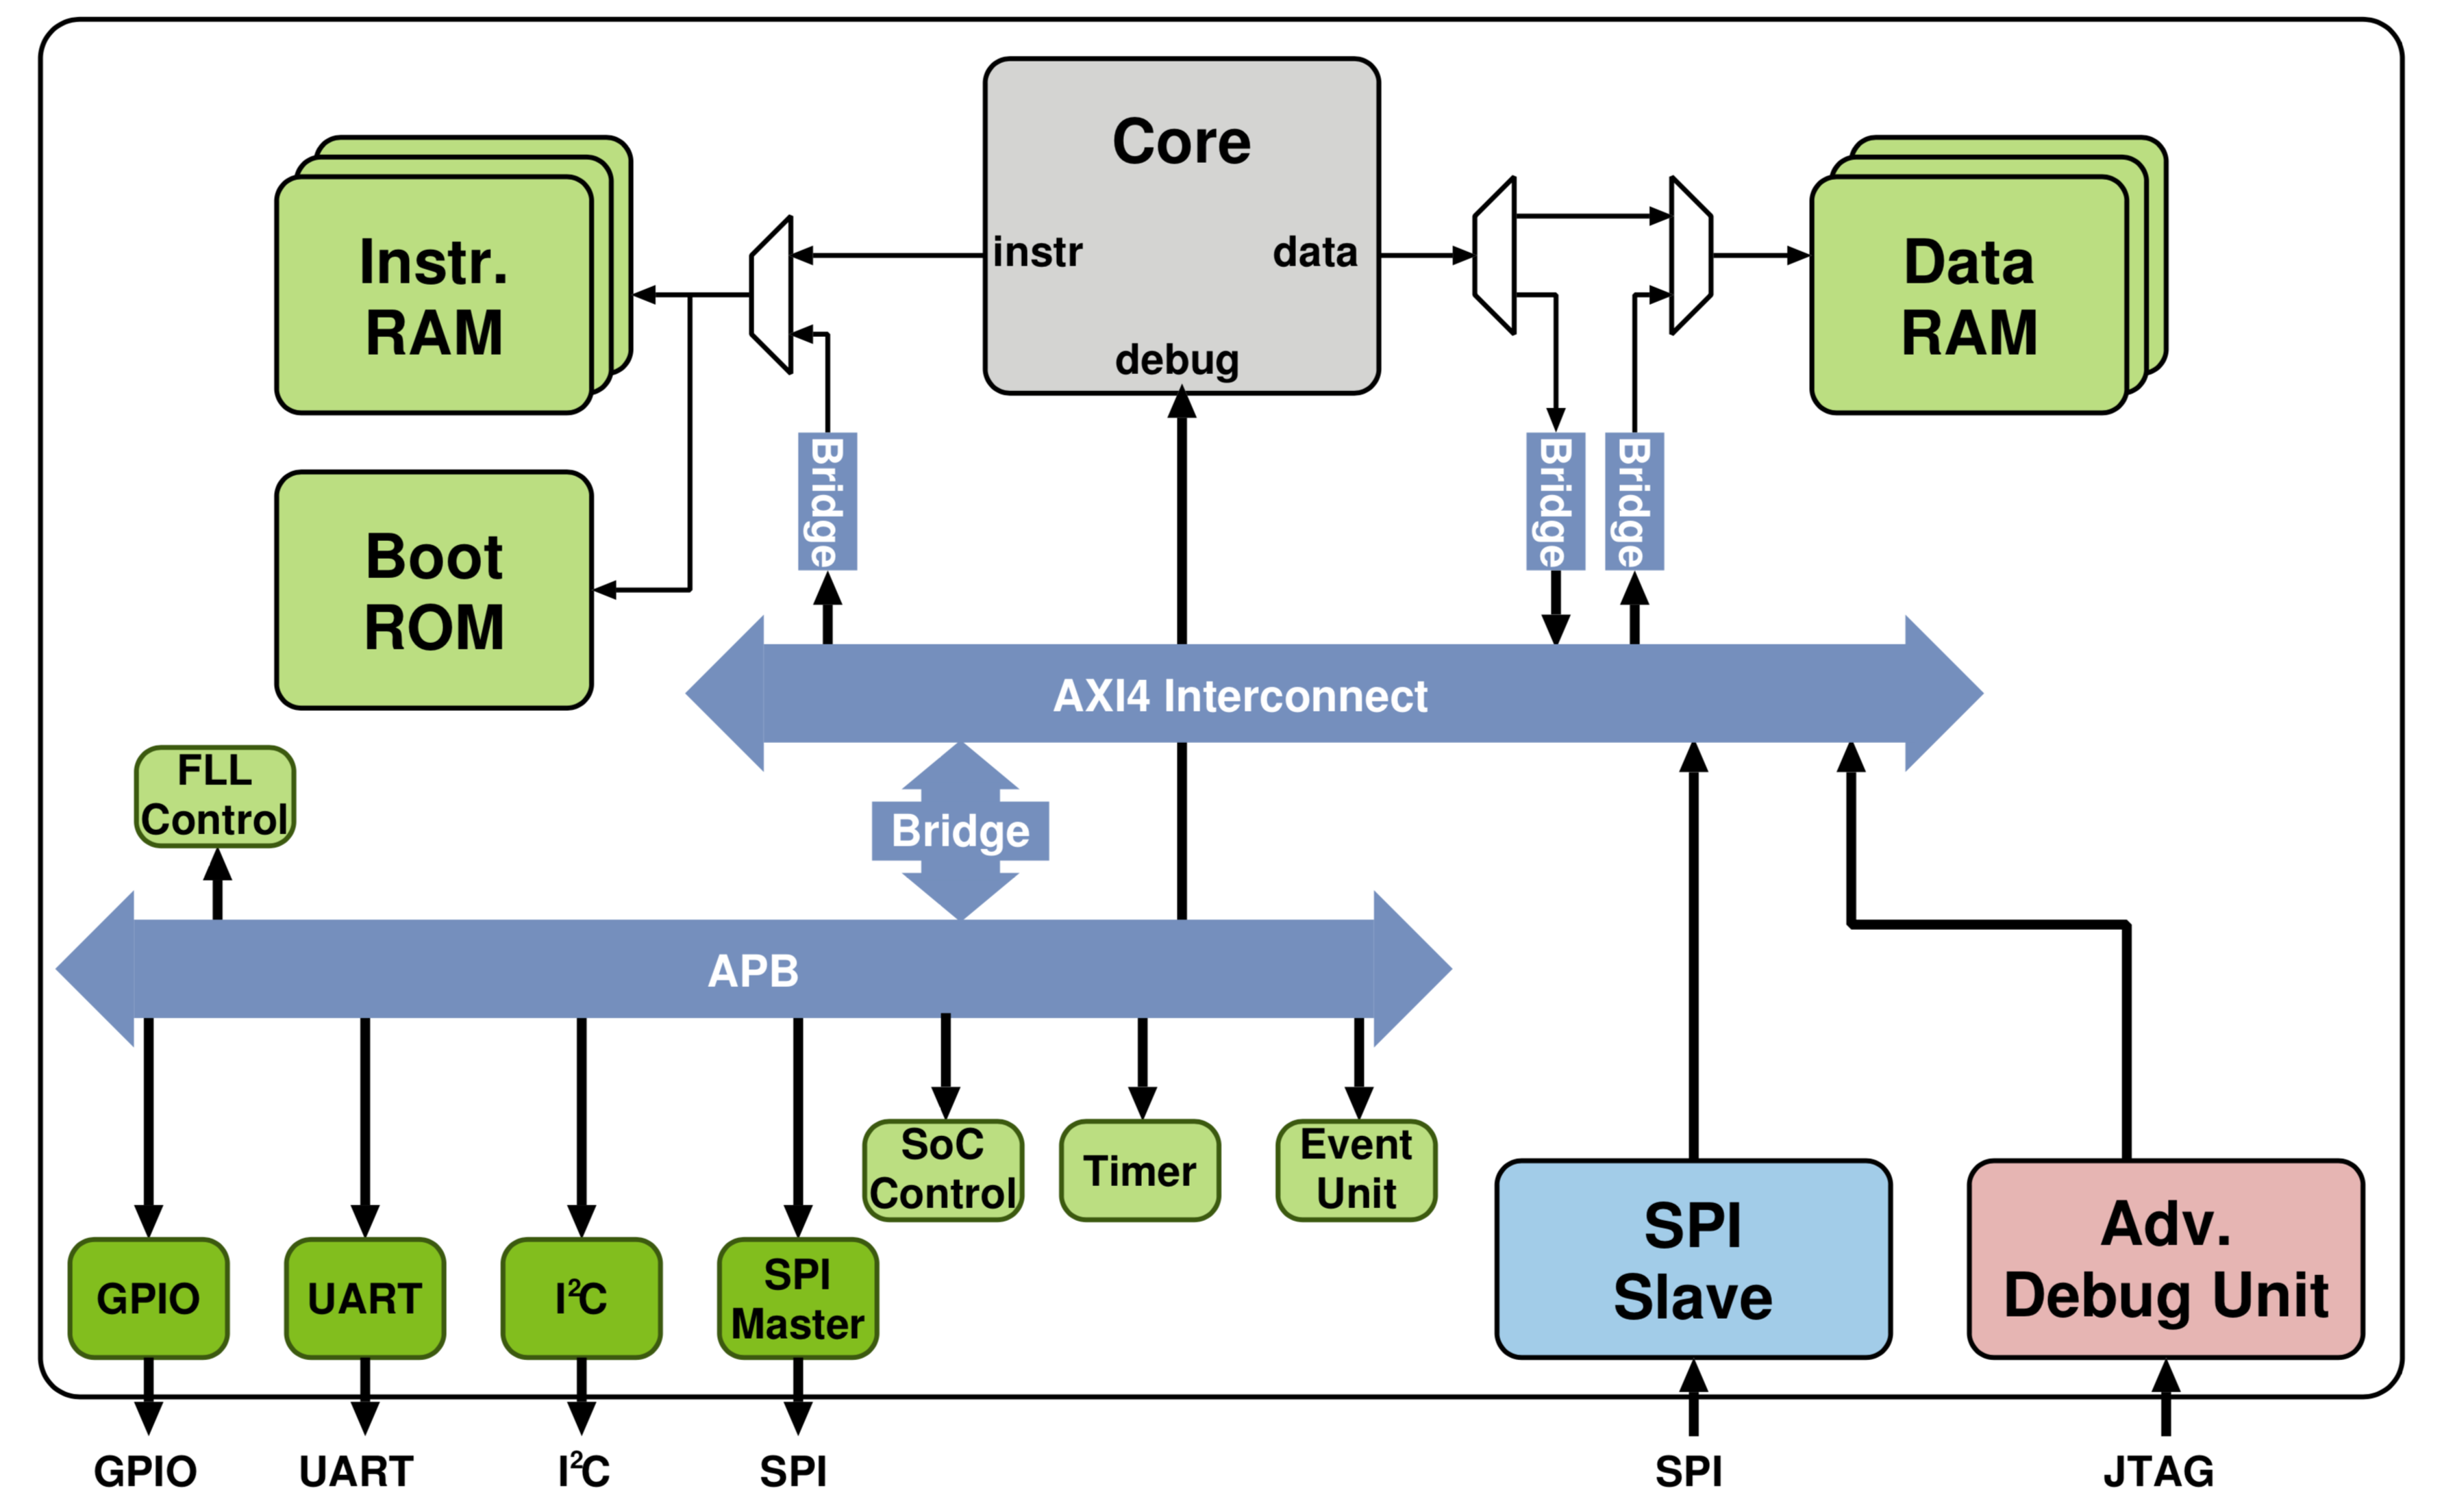
\includegraphics[height=2.2 in]{./pics/PULPino_System_Architecture}
\caption{Pulpino system architecture}
\label{fig:PULPinoSystemArchitecture}
\end{figure}
}

%	32-bit processors


%%%%%%%%%%%%%%%%%%%%%%%%%%%%%%%%%%%%%%%%%%%%%%
%	Memory Map
\section{Memory Map}

%	Slide 1
\frame
{
	\frametitle{Memory Map}

%	\begin{itemize}
%	\item Cyber-physical system design
%	\item Implement a memory game on the {\it Arduino} platform: %\vspace{-0.3cm}
%		\begin{itemize} %\itemsep -2pt
%		\item Implement simple analog circuit design on a breadboard
%		\item Connect breadboard to the {\it Arduino} platform
%		\item Program the microcontroller on the {\it Arduino} platform
%		\end{itemize}
%	\item Play the memory game
%	\item Repeat previous steps ad infinitum until you get bored.
%	\end{itemize}

\begin{figure}[h]
\centering 
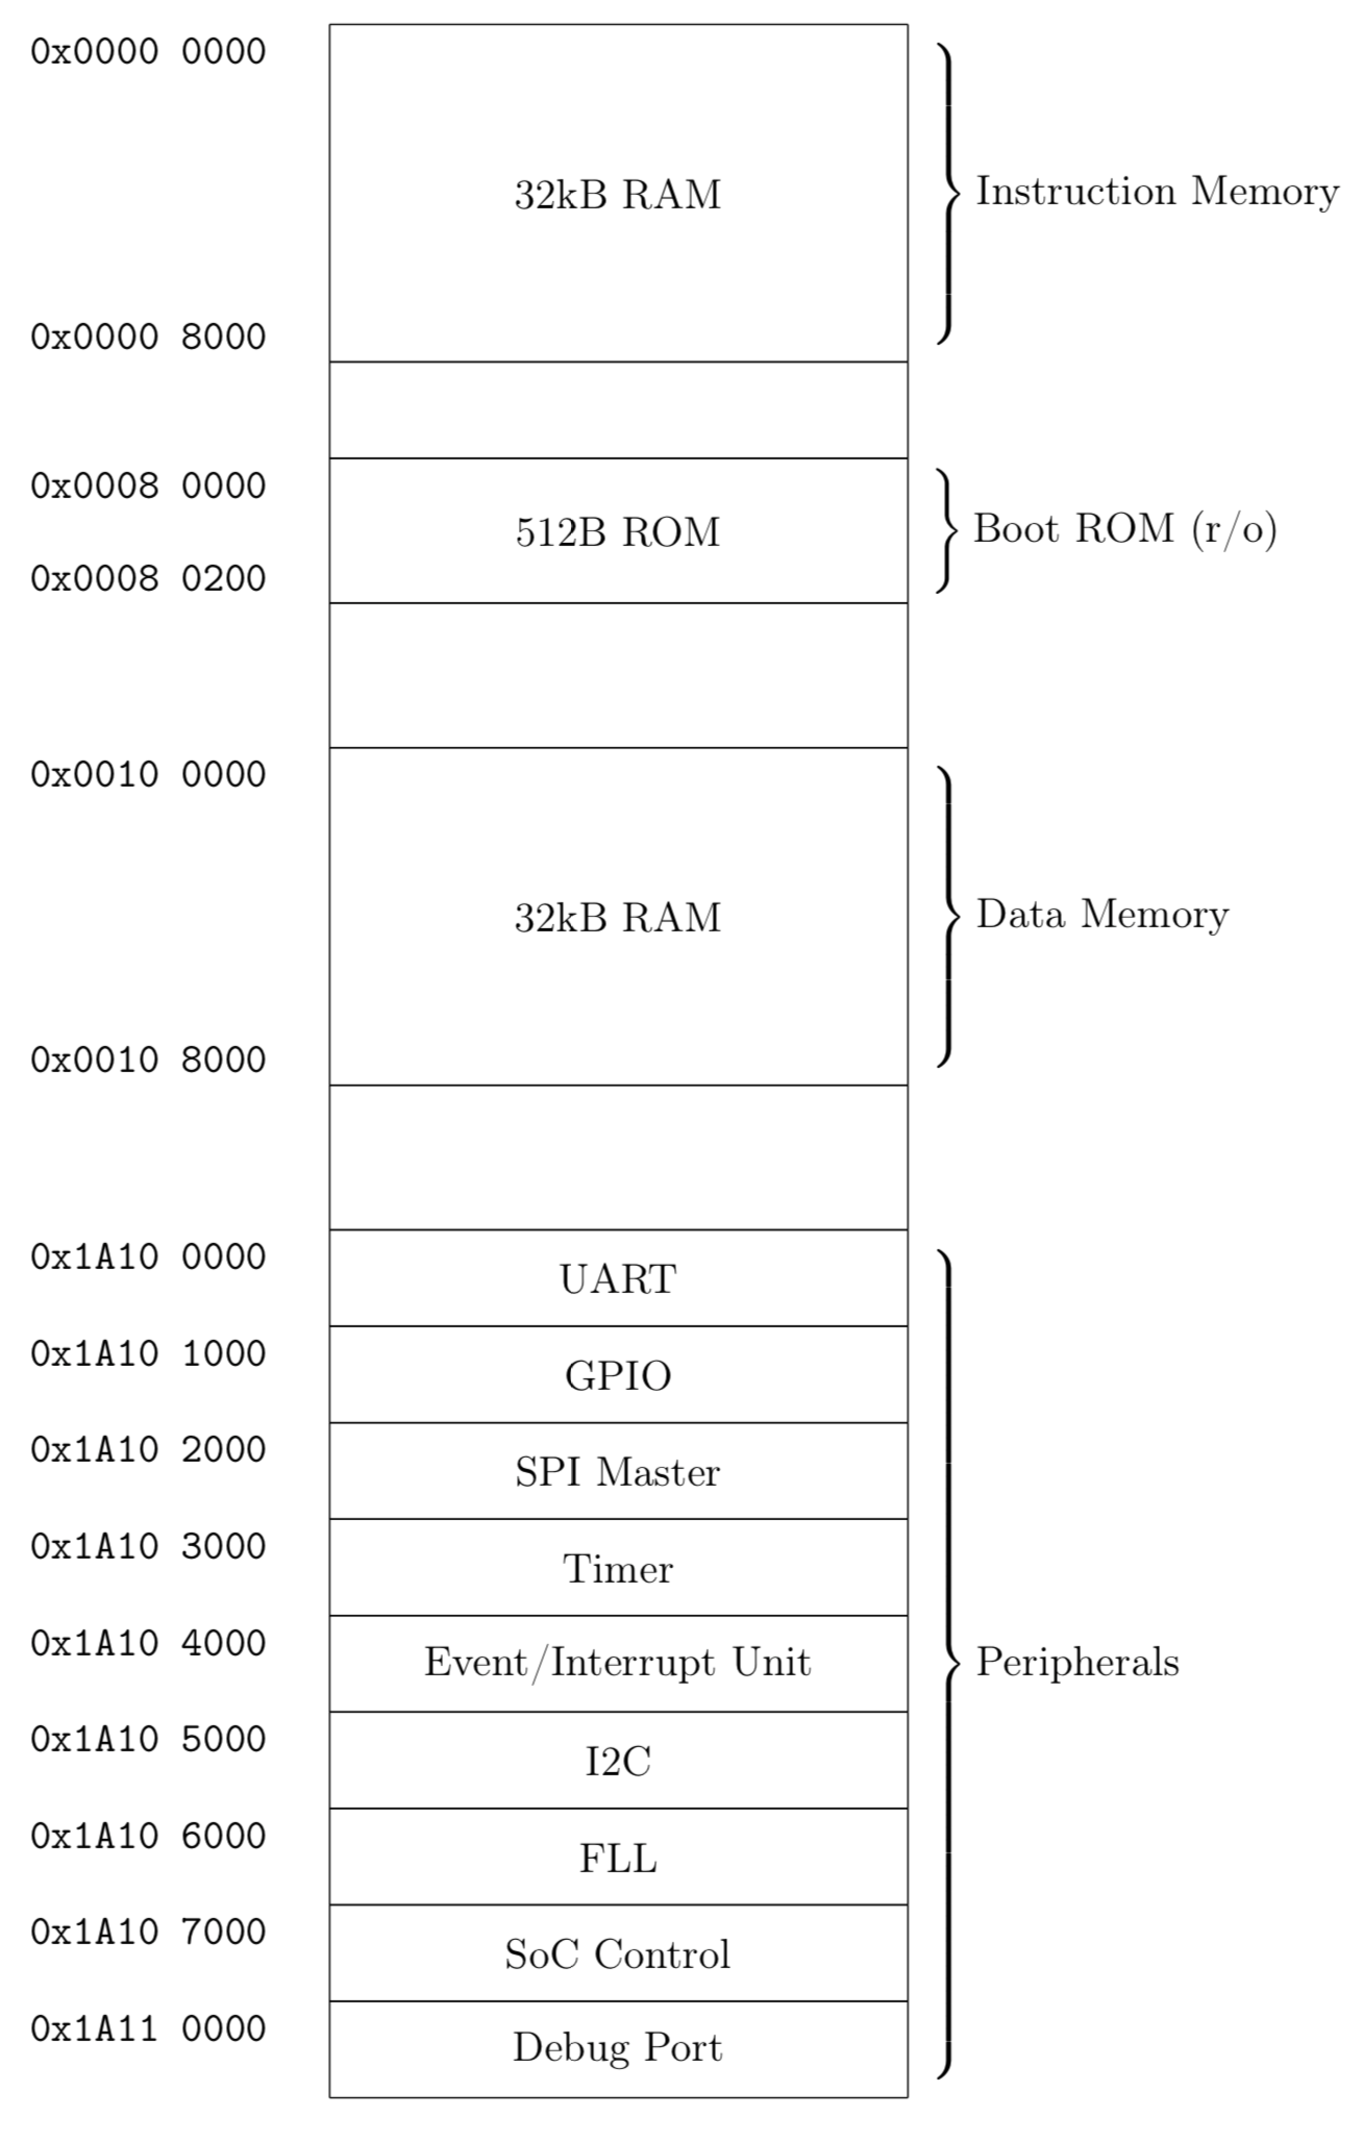
\includegraphics[height=2.2 in]{./pics/Pulpino_Memory_Map}
\caption{Pulpino memory map}
\label{fig:PulpinoMemoryMap}
\end{figure}
}





%%%%%%%%%%%%%%%%%%%%%%%%%%%%%%%%%%%%%%%%%%%%%%
%	Topics in Hardware Security
\section{Topics in Hardware Security}



%	Slide #1
\frame
{
	\frametitle{Topics in Hardware Security (1)}

	Supply-side attacks for supply-chain hardware security \begin{itemize}
	\item hardware backdoor attacks
		\begin{itemize}
		\item hardware trojans, or malicious circuits
			\begin{itemize}
			\item add, modify, or delete data
			\item do something unintended
			\item don't do something intended
			\end{itemize}
		\item malicious firmware (insertion \& execution)
		\item Test and verification features
			\begin{itemize}
			\item Advanced Debug Unit (for JTAG)
			\item Debug port for APB-based memory mapped debugging
			\end{itemize}
		\end{itemize}
	\end{itemize}
}


%	Slide #2
\frame
{
	\frametitle{Topics in Hardware Security (2)}

	More supply-side attacks for supply-chain hardware security \begin{itemize}
	\item Attackers
		\begin{itemize}
		\item third-party RTL vendors
		\item disgruntled employees of IC design team
		\item EDA vendors can produce malicious/defective circuits
		\item Everyone in downstream of supply-chain are liable
		\end{itemize}
	\item Hardware piracy
	\item Counterfeit attack
	\end{itemize}
}




%%%%%%%%%%%%%%%%%%%%%%%%%%%%%%%%%%%%%%%%%%%%%%
%	Attack Scenario for \dots
\section{Attack Scenario for \dots}


%	Slide 1
\frame
{
	\frametitle{High-level attack scenarios (1)}

	\begin{itemize}
	\item Assume that Boot ROM contains initial values
		\begin{itemize}
		\item Access to Boot ROM
			\begin{itemize}
			\item Read from data memory (RAM) instead.
			\item Read ``garbage'' (maliciously inserted instructions) from instruction memory (RAM) instead.
			\item Read data standard input port instead (software-driven process/operation).
			\item Unauthenticated read access to boot ROM outside of boot up procedure.
			\end{itemize}
		\item Writing to Boot ROM should always be forbidden.
		\end{itemize}
	\item If authentication is required for read access to the boot ROM, 
		\begin{itemize}
		\item Only the authorized read access (in normal mode or debug/testing mode) during boot up or rebooting is allowed.
		\item Else, forbid read access outside of booting up or rebooting is allowed.
		\end{itemize}
	\end{itemize}
}


%	Slide 2
\frame
{
	\frametitle{High-level attack scenarios (2)}

	Read/Write access data in data/instruction RAM via input/output ports, without authentication (1):
	\begin{itemize}
	\item Input/Output (I/O) ports and buses to consider
		\begin{itemize}
		\item General-purpose input/output (GPIO)
		\item UART
		\item SPI Master / AXI Master, and SPI Slave; see Serial Peripheral Interface bus (SPI)
		\end{itemize}
	\item Read ``important'' data that I should not access, without authentication; e.g., keys for encryption/decryption.
	\end{itemize}
}





%	Slide 3
\frame
{
	\frametitle{High-level attack scenarios (3)}

	Read/Write access data in data/instruction RAM via input/output ports, without authentication (2):
	\begin{itemize}
	\item Fill up the data and/or instruction RAM with garbage, and/or malicious data and instructions.
		\begin{itemize}
		\item Invalid instructions fetched and decoded by the RISV-V processor(s) should result in raising an illegal instruction exception at address 0x00000084 (\S2.1, Table 2.1, page 7 of the datasheet)
		\end{itemize}
	\item Invalid memory access (i.e., areas not specified in the memory map) shall raise an invalid memory access exception at address 0x0000008C (\S2.1, Table 2.1, page 7 of the datasheet).
	\item Load malicious firmware to the instruction RAM:
		\begin{itemize}
		\item add, modify, or delete data
		\item do something unintended
		\item don't do something intended
		\end{itemize}
	\end{itemize}
}






%%%%%%%%%%%%%%%%%%%%%%%%%%%%%%%%%%%%%%%%%%%%%%
%	Attack Scenario for Hardware Trojans
\section{Attack Scenario for Hardware Trojans}

%	Slide 1
\frame
{
	\frametitle{Abstract Attack Scenario for Hardware Trojans or Malicious Circuits (1)}

	\begin{itemize}
	\item Attack objectives/goals, or 
		\begin{itemize}
		\item read (G1), add (G2), modify (G3), or delete (G4) data
		\item do something unintended (G5)
		\item don't do something intended (G6)
		\end{itemize}
	\item Man-in-the-middle attack: G1, G2, G3, G4, G5, G6
	\item Backdoor attack: G1, G2, G3, G4, G5, G6
	\item Eavesdropping attack: G1
	\item Privilege escalation: G1, G2, G3, G4, G5, G6
	\item Side-channel attack: G1, G2, G3, G4, G5, G6
	\end{itemize}
}










%%%%%%%%%%%%%%%%%%%%%%%%%%%%%%%%%%%%%%%%%%%%%%
%	Attack Scenario for Hardware Test and Verification Features
\section{Attack Scenario for Hardware Test and Verification Features}

%	Slide 1
\frame
{
	\frametitle{Abstract Attack Scenario for Hardware Test and Verification Features (1)}

	\begin{itemize}
	\item Trade-off between hardware security and testability/verifiability
	\item An attacker ({\it Mallory} $[$Wikipedia contributors 2016$]$) can exploit the observability and controllability of the system that VLSI verification and testing need.
	\item {\it Mallory} exploits the observability and controllability of the system, via its debug and test modes/features.
	\end{itemize}
}

%	Slide 2
\frame
{
	\frametitle{Abstract Attack Scenario for Hardware Test and Verification Features (2)}

\begin{figure}[h]
\centering 
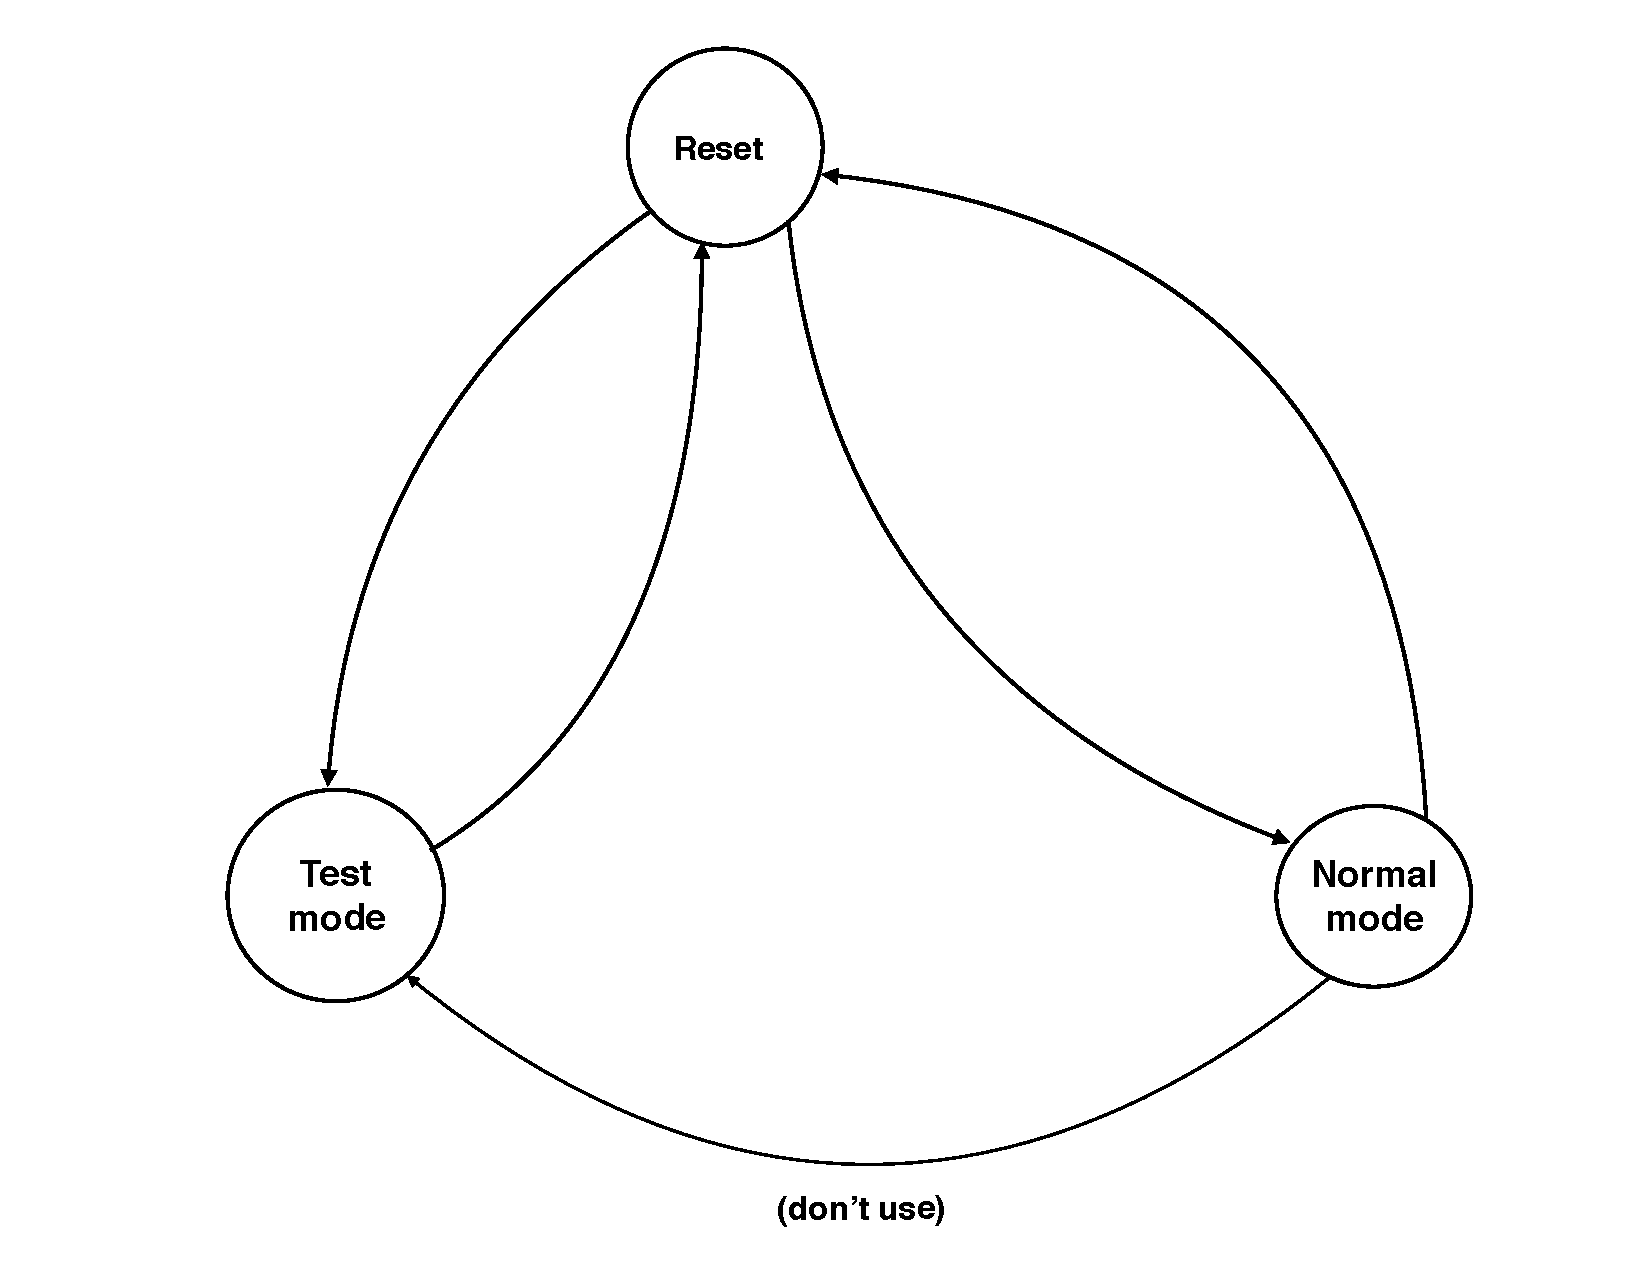
\includegraphics[height=2.2in]{./pics/no_reset_soln}
\caption{Unsafe Finite State Machine Model of a System-Under-Test}
\label{fig:NoResetSolution}
\end{figure}

}


%	Slide 3
\frame
{
	\frametitle{Abstract Attack Scenario for Hardware Test and Verification Features (3)}

\begin{figure}[h]
\centering 
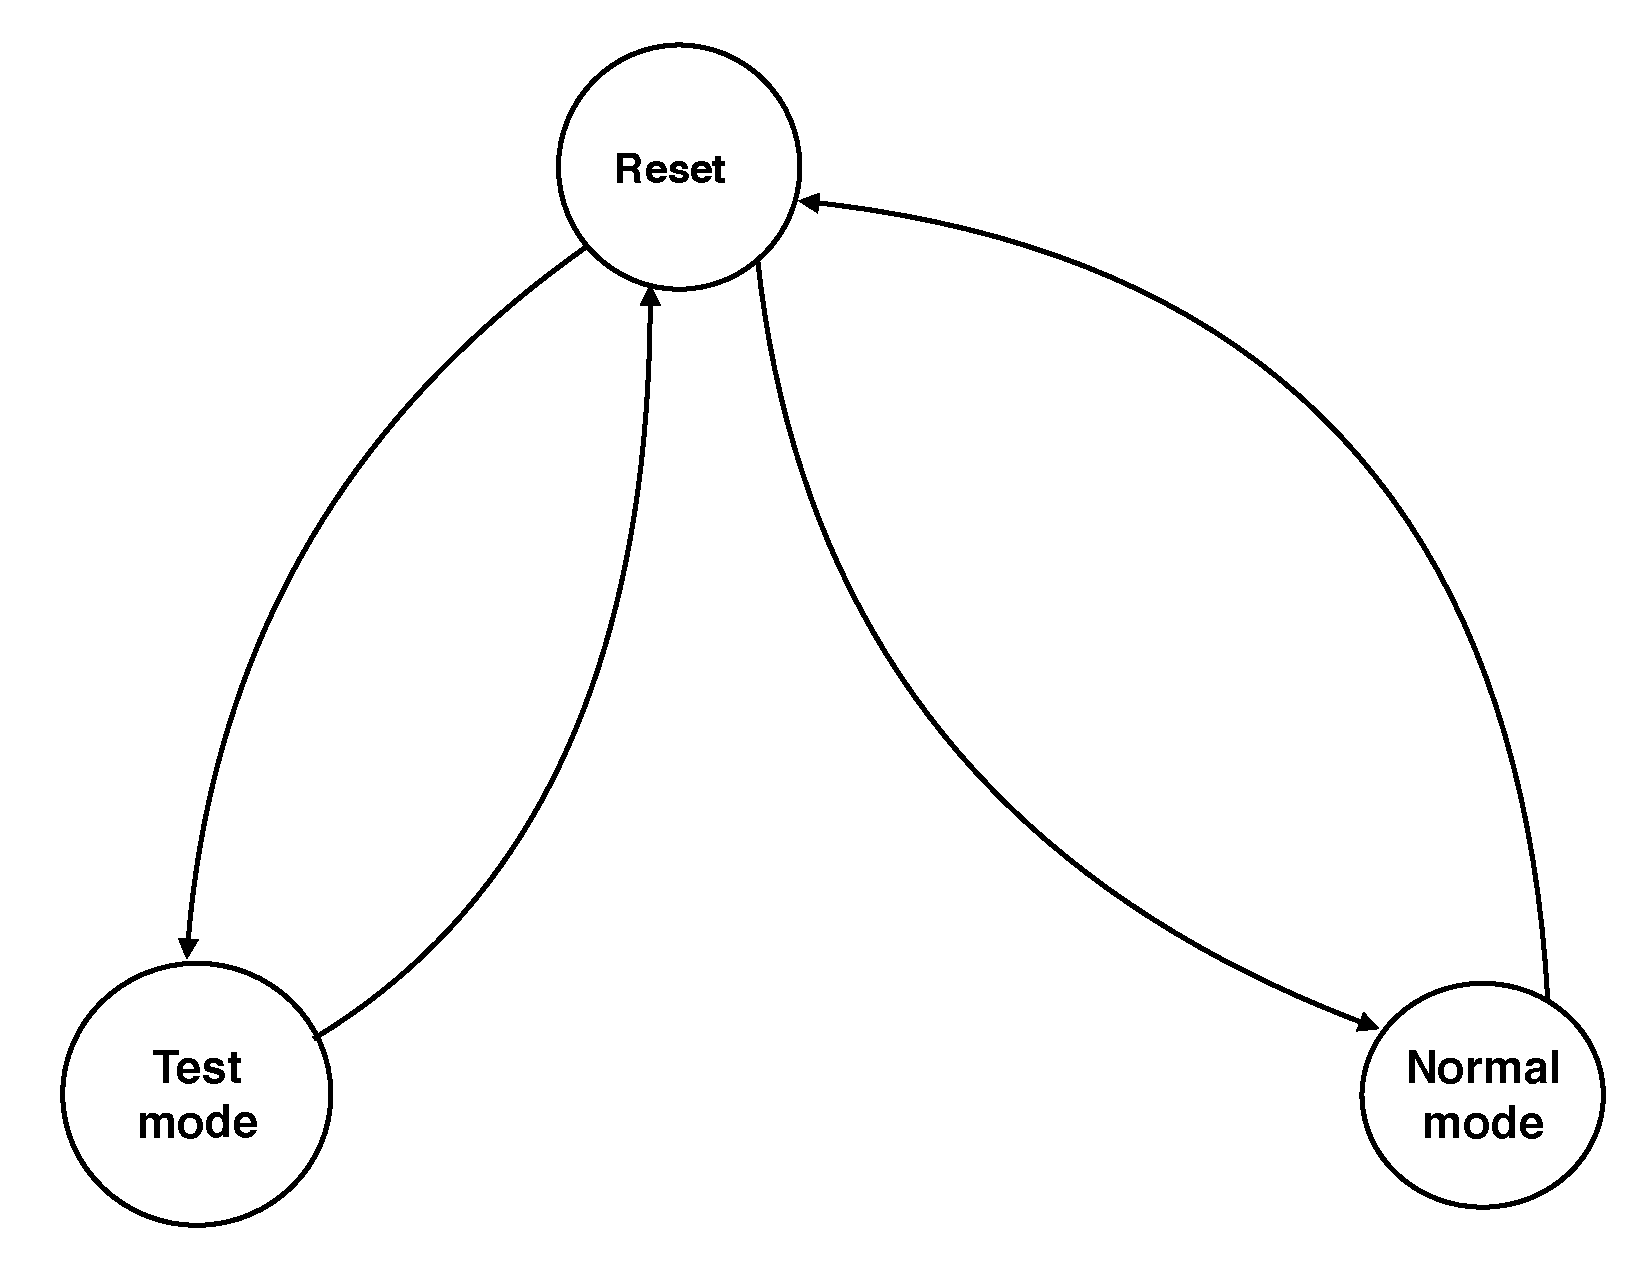
\includegraphics[height=2.2in]{./pics/reset_soln}
\caption{Safer Finite State Machine Model of a System-Under-Test}
\label{fig:ResetSolution}
\end{figure}

}






%	Advanced Microcontroller Bus Architecture (AMBA) Advanced Peripheral Bus (APB).
%	The ARM Advanced Microcontroller Bus Architecture (AMBA) is an open-standard, on-chip interconnect specification for the connection and management of functional blocks in system-on-a-chip (SoC) designs. 







%	Unified Extensible Firmware Interface (UEFI)

%	References:
% https://www.dropbox.com/sh/2ufe9f8viygf2oj/AAAMfmOzoqeHtWHuLsH89OZQa/????dl=0&preview=Ecall_06302017.pptx
% https://www.youtube.com/watch?v=UPHEkz_rHTY
%	ECALL is a user-level instruction in the RISC-V ISA; it is used to make a request to the supporting execution environment (OS), and to implement syscalls in Linux.


%	Slide 4
\frame
{
	\frametitle{Attack Scenario for JTAG \#1: Switch directly from normal mode to test mode (1)}

	\begin{itemize}
	\item Set input signal tms (test mode select), so that it transits from the ``idle'' state/mode to the ``test'' state/mode, in the state machine of the test access port (TAP) controller (or JTAG state machine).
		\begin{itemize}
		\item At ``idle'' state, {\it TMS = 0} will cause the TAP controller to remain the the ``idle'' state.
		\item From the ``idle'' state, {\it TMS = 1} will cause the TAP controller to transit to the ``run test'' state, without going to the ``test logic reset'' state.
		\end{itemize}
	\item According to Prof. Jeyavijayan (JV) Rajendran, an updated JTAG standard requires/forces the TAP controller to transit from ``idle'' state to the ``run test'' state, via the ``reset'' state.
		\begin{itemize}
		\item See Table 10.1 about the IEEE 1149 standard family $[$Wang 2006$]$
		\end{itemize}
	\end{itemize}

%	\begin{itemize}
%	\item Set input signals:
%		\begin{itemize}
%		\item trstn (test reset, active low): 
%		\item tck (test clock)
%		\item tms (test mode select)
%		\item tdi (test data input)
%		\end{itemize}
%	\item Read output signals:
%		\begin{itemize}
%		\item tdo (test data output)
%		\item AXI Master ()
%		\end{itemize}
%	\end{itemize}

% References:
%	https://www.electronics-notes.com/articles/test-methods/boundary-scan-jtag-ieee1149/jtag-interface-tap-test-access-port-connector.php
}




%	Slide 5
\frame
{
	\frametitle{Attack Scenario for JTAG \#1: Switch directly from normal mode to test mode (2)}

\begin{figure}[h]
\centering 
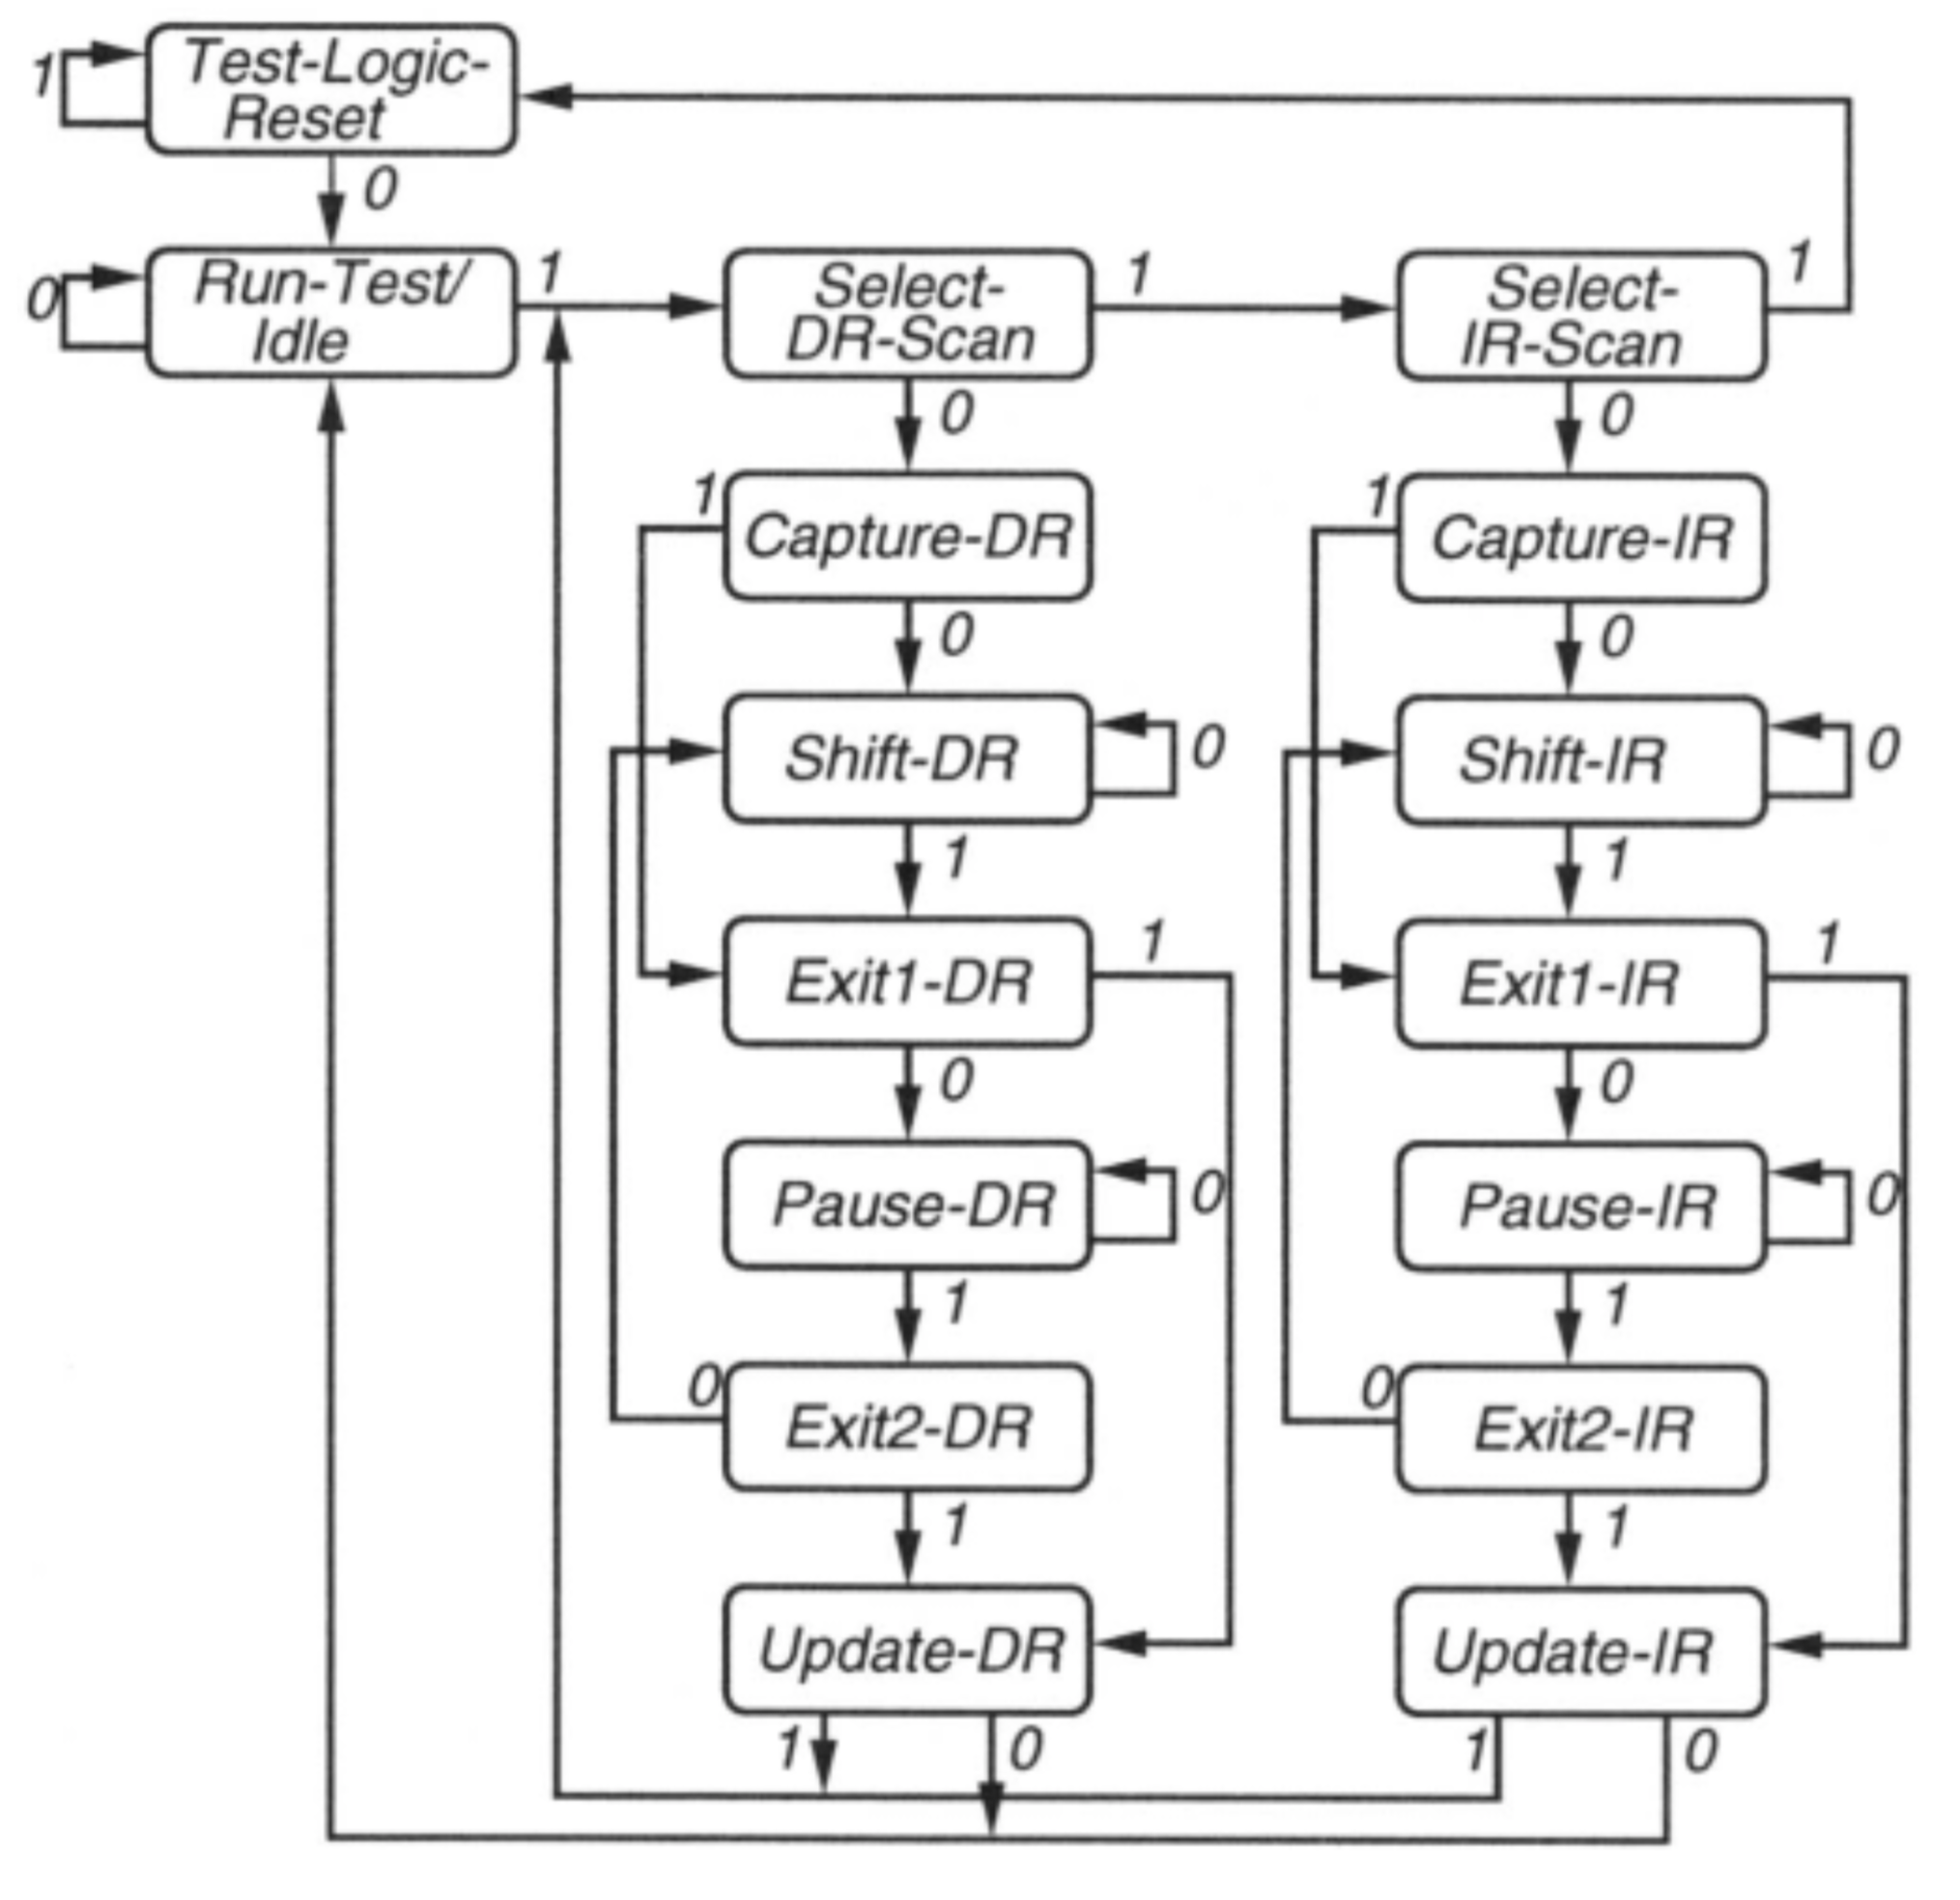
\includegraphics[height=2.0in]{./pics/jtag_tap_controller_Bushnell2000}
\caption{Finite state machine of the JTAG test access port (TAP) controller $[$Bushnell 2000, \S16.2.1, Figure 16.11, pp. 558$]$}
\label{fig:JTAGTAPcontrollerBushnell2000}
\end{figure}
}

%	Slide 6
\frame
{
	\frametitle{Attack Scenario for JTAG \#1: Switch directly from normal mode to test mode (3)}

\begin{figure}[h]
\centering 
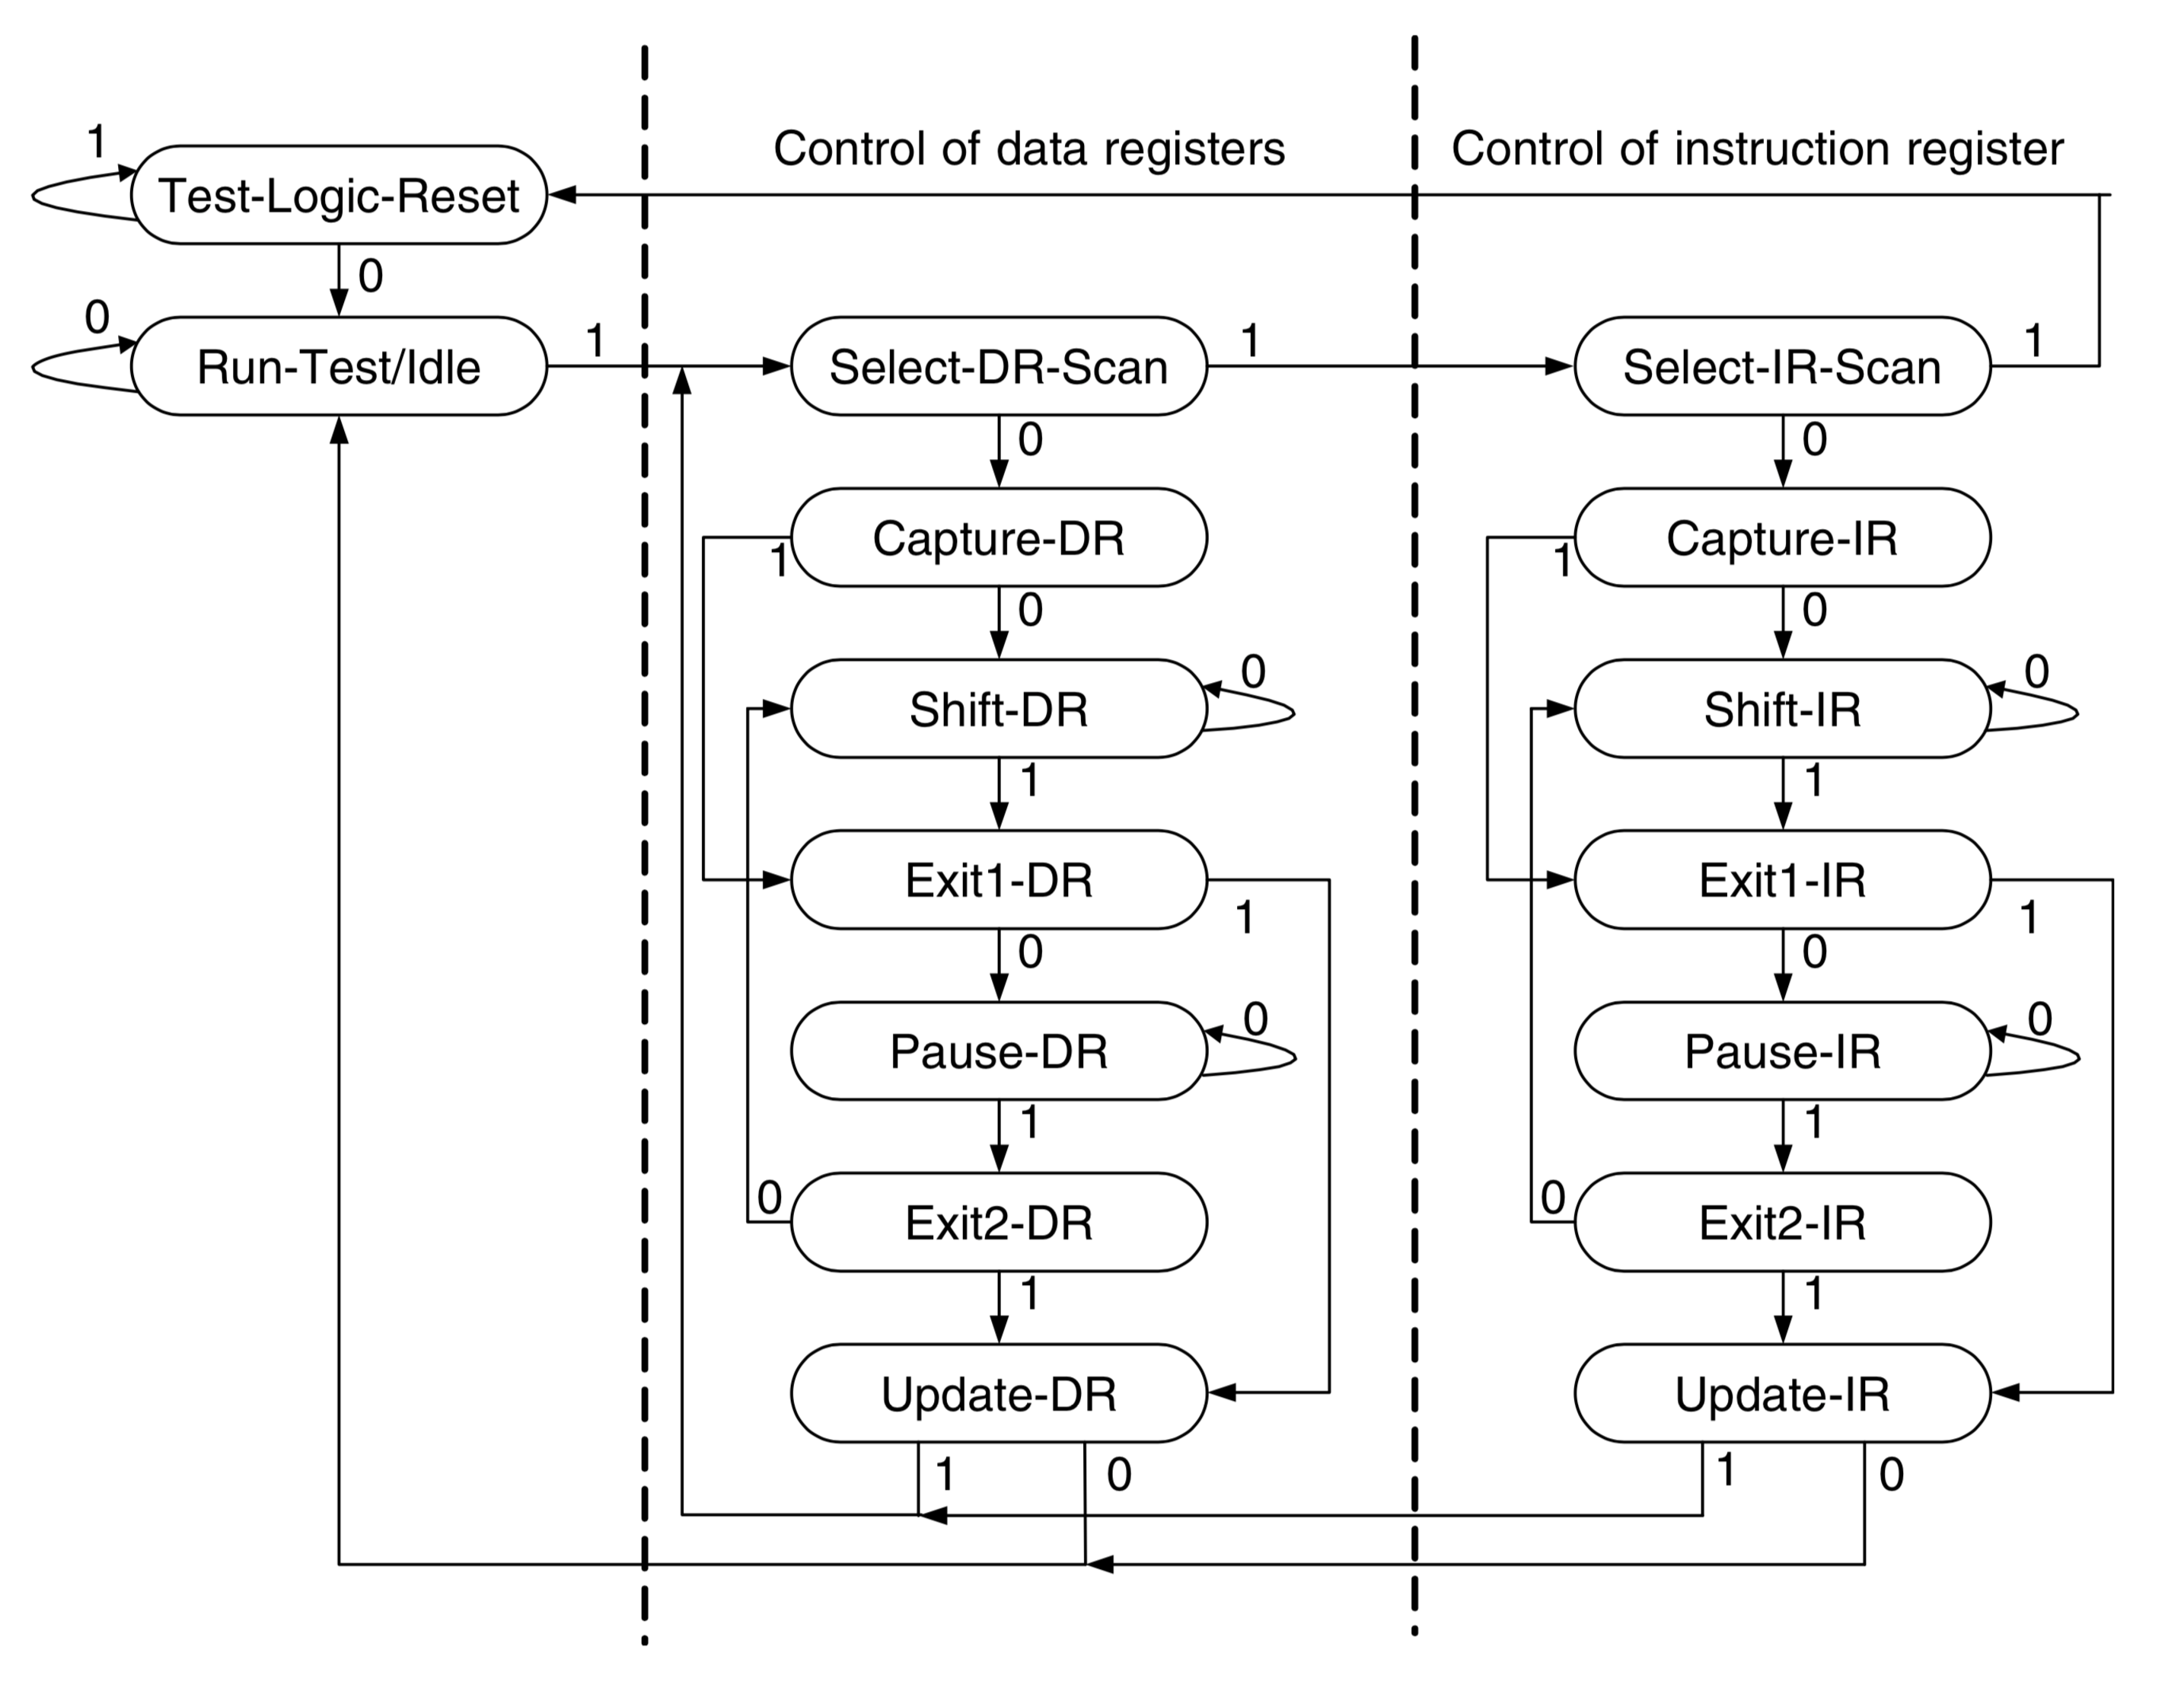
\includegraphics[height=2.0in]{./pics/jtag_tap_controller_Wang2006b}
\caption{Finite state machine of the JTAG test access port (TAP) controller $[$Wang 2006, \S10.2.5, Figure 10.7, pp. 567$]$}
\label{fig:JTAGTAPcontrollerWang2006b}
\end{figure}
}

%	Also, see \cite[\S9.10.5.1, Figure 9.53, pp. 406]{Abramovici1990}.
%	Miron Abramovici, Melvin A. Breuer, and Arthur D. Friedman, ``Digital Systems Testing and Testable Design,'' Revised Printing, IEEE Press, New York, NY, 1990.




%	Slide 7
\frame
{
	\frametitle{Attack Scenario for JTAG \#2: Access Boot ROM}

	\begin{itemize}
	\item Assume that Boot ROM contains initial values
	\item Without authentication, access the boot ROM.
		\begin{itemize}
		\item If this is feasible, it may be a security bug if security-related functions are performed during booting/rebooting.
		\end{itemize}
	\item With authentication, modify the boot ROM.
		\begin{itemize}
		\item This attempt should fail.
		\item Else, it is a security bug, since malicious instructions can be inserted into the boot ROM.
		\end{itemize}
	\end{itemize}
}








%	Slide 7
\frame
{
	\frametitle{Attack Scenario for JTAG \#2: Access Instruction and Data RAMs}

	\begin{itemize}
	\item Without authentication, scan the data from the instruction RAM to the instruction register (IR), and subsequently scan the instructions out (to an output data acquisition device).
		\begin{itemize}
		\item If this is feasible, it may be a security bug if security-related functions are performed during operation of the {\it Pulpino} platform.
		\end{itemize}
	\item Without authentication, scan the data from the data RAM to the data registers (DR), and subsequently scan the data out (to an output data acquisition device).
		\begin{itemize}
		\item If this is feasible, it may be a security bug if private keys (for encryption/decryption) are stored in the data RAM without encryption.
		\end{itemize}
	\item With authentication, the aforementioned tasks should fail.
	\end{itemize}
}









%	Slide 8
\frame
{
	\frametitle{Attack Scenario for Debug Port}

	\begin{itemize}
	\item In debug mode
		\begin{itemize}
		\item Insert malicious firmware into instruction RAM
			\begin{itemize}
			\item Unauthorized access to, addition to, modification of, or deletion of data
			\item To do something unintended
			\item To avoid doing something intended
			\end{itemize}
		\end{itemize}
	\item Gain unauthorized access to data
		\begin{itemize}
		\item Add, modify, or delete data
		\item Send data to output device
		\end{itemize}
	\item When authorized, ensure that data cannot be modified or accessed inappropriately.
	\end{itemize}



}








%%%%%%%%%%%%%%%%%%%%%%%%%%%%%%%%%%%%%%%%%%%%%%
%	Attack Scenario Regarding Privileges and Race Conditions
\section{Attack Scenario Regarding Privileges and Race Conditions}

%	Slide 1
\frame
{
	\frametitle{Attack Scenario Regarding Privileges}

	\begin{itemize}
	\item Hardware trojan can generate an interrupt to write value into a Control/Status Register (CSR), via I$^{2}$C (Inter-Integrated Circuit).
	\item This value may not be the true/actual value of the CSR and/or interrupt handler.
	\item $[$Khabarov 2015$]$
	\end{itemize}
}

%	Fence instruction
% https://stackoverflow.com/questions/26374435/what-is-meant-by-the-fence-instruction-in-the-risc-v-instruction-set
%	Mobile Industry Processor Interface, MIPI
%	Control/Status Register, CSR



%	Slide 2
\frame
{
	\frametitle{Attack Scenario Regarding Race Conditions}

	\begin{itemize}
	\item Use the frequency lock loop (FLL) ``to generate clock frequencies faster [or slower???] than the reference clock frequency'' (Ghada Dessouky, Hack DAC '18 {\it Slack} channel)
	\item Can cause race conditions and race hazards
	\item Can cause timing violations of registers (i.e., flip-flops and latches)
	\item Cause the system to do something unintended
	\end{itemize}
}

%	from https://hack-dac18.slack.com/messages
%	Ghada Dessouky [4:08 AM], February 28, 2018
%	Hack DAC '18 {\it Slack} channel
%	``[FLL] stands for frequency locked loop - usually used to generate clock frequencies faster than the reference clock frequency''
%	What does the FLL refer to in the "PULPino: Datasheet", shown in Figure 1.1 (page 4) and Figure 2.1 (page 6)?




%%%%%%%%%%%%%%%%%%%%%%%%%%%%%%%%%%%%%%%%%%%%%%
%	Inadequately Addressed Hardware Security Challenges
\section{Inadequately Addressed Hardware Security Challenges}

%	Slide 1
\frame
{
	\frametitle{Inadequately Addressed Hardware Security Challenges}

	Hardware trojans, or malicious circuits, that:
	\begin{itemize}
	\item Do something unintended (not in the design specifications).
	\item Carry out unauthorized access, addition, modification, or deletion of data
	\item Don't do something intended.
	\item Check the connections (i.e., I/O ports) of buses (i.e., APB \& AXI interconnect) for unspecified connections.
	\end{itemize}
}




%%%%%%%%%%%%%%%%%%%%%%%%%%%%%%%%%%%%%%%%%%%%%%
%	How to Detect Hardware Trojans
\section{How to Detect Hardware Trojans}

%	Slide 1.
\frame
{
	\frametitle{How to Detect Hardware Trojans (1)}

	\begin{itemize}
	\item Walk through code (i.e., code walkthrough)\dots Tedious.
	\item Use verification-based techniques to detect security bugs.
		\begin{itemize}
		\item Tailor these techniques to specific VLSI circuit/system designs, or family of such designs.
		\item {\it Bring the FSM to an invalid state???}
		\end{itemize}
	\item Proof-carrying code techniques, which were initially developed for software security vulnerabilities
		\begin{itemize}
		\item Use divide \&\ conquer to partition hardware system into RTL/TLM code segments
		\item The arbitrator checks each RTL/TLM component (or code segment) with its corresponding theoretical proof.
		\end{itemize}
	\end{itemize}
}




%	Slide 2.
\frame
{
	\frametitle{How to Detect Hardware Trojans (2)}

	Modify techniques for mitigating hardware trojans at the circuit- (i.e., cell-/gate- or logic level) or physical- (i.e., layout) levels \begin{itemize}
	\item Make use of software redundancy to use a hardware component (e.g., ALU/adder) in redundant ways and compare their results.
		\begin{itemize}
		\item If the component doesn't behave as expected, a trojan exists; can't prove information leaks.
		\item Composability problem: Hardware trojan may only be activated when the components are integrated to form the composed system.
		\item Given code and proof, we can check if there exists vulnerabilities. But, we can't attest to anything outside the proof, such as the absence of data modification, system/hardware reset, and/or information leakage.
		\end{itemize}
	\end{itemize}
}



%	Slide 3.
\frame
{
	\frametitle{How to Detect Hardware Trojans (3)}

	\begin{itemize}
	\item Compare different implementations of a component for the {\it PULPino} system (e.g., ALU/adder for the RISC-V ISA)
		\begin{itemize}
		\item The same input is given to these different implementations.
		\item The output of these different implementations is given to a majority gate (i.e., use majority voting).
		\item Components that yield a different output from the majority of the components have hardware trojans.
		\item That is, use techniques from fault tolerance for detecting hardware trojans. 
		\item While we cannot use TLM/RTL models from others, we can create our own TLM/RTL models (using {\it SystemC}, {\it Verilog}, and/or {\it Chisel}) for components of the {\it PULPino} system.
		\end{itemize}
	\end{itemize}
}





%	Slide 4.
\frame
{
	\frametitle{How to Detect Hardware Trojans (4)}

	\begin{itemize}
	\item Use the aforementioned software redundancy technique to determine which hardware component went bad, and when and how (i.e.., sequence of input patterns) did it go bad.
	\item Additional comments on hardware security
		\begin{itemize}
		\item In functional verification, we know what to check for.
		\item In security verification, we don't know what to check for.
		\item See Church thesis, Rice theorem, \dots
		\end{itemize}
	\end{itemize}
}







%%%%%%%%%%%%%%%%%%%%%%%%%%%%%%%%%%%%%%%%%%%%%%

\section{References}

%	Slide 1
\frame
{
	\frametitle{References (1)}

	\begin{itemize}
	\item $[$Wikipedia contributors 2016$]$ Wikipedia contributors, ``Alice and Bob,'' in {\it Wikipedia, The Free Encyclopedia: Cryptographic protocols}, Wikimedia Foundation, San Francisco, CA, February 28, 2018. Available online at: \url{https://en.wikipedia.org/wiki/Alice_and_Bob}; last accessed on October 26, 2016.
	\item $[$Khabarov 2015$]$ Sergey Khabarov, answer to ``What is meant by the FENCE instruction in the RISC-V instruction set?,'' Stack Exchange Inc., New York, NY, November 23, 2015. Available online from {\it Stack Exchange Inc.: Stack Overflow: Questions} at: \url{https://stackoverflow.com/questions/26374435/what-is-meant-by-the-fence-instruction-in-the-risc-v-instruction-set}; March 16, 2016 was the last accessed date.
	\end{itemize}
}



%	Slide 2
\frame
{
	\frametitle{References (2)}

	\begin{itemize}
	\item $[$Bushnell 2000$]$ Michael L. Bushnell and Vishwani D. Agrawal, ``Essentials of Electronic Testing for Digital, Memory, and Mixed-Signal {VLSI} Circuits,'' in {\it Frontiers in Electronic Testing} series, Vol. 17, Springer Science+Business Media, {Inc.}, New York, NY, 2000. DOI:10.1007/b117406.
	\item $[$Wang 2006$]$ {Laung-Terng} Wang, {Cheng-Wen} Wu, and Xiaoqing Wen, ``{VLSI} Test Principles And Architectures: Design for Testability,'' in {\it The Morgan Kaufmann Series in Systems on Silicon}, Morgan Kaufmann, San Francisco, CA, 2006.
	\end{itemize}
}








%%%%%%%%%%%%%%%%%%%%%%%%%%%%%%%%%%%%%%%%%%%%%%

\section{Questions}

\frame
{
	\frametitle{Questions}

	\begin{itemize}
	\item Is authentication required for read access to the boot ROM?
	\end{itemize}
}


%	Debug mode. Stall the core. Testbench.






%%%%%%%%%%%%%%%%%%%%%%%%%%%%%%%%%%%%%%%%%%%%%%
%\section{References}
%
%\frame
%{
%	\frametitle{References}
%
%%	\begin{itemize}
%%	\item \cite{Weng2011}
%%	\end{itemize}
%%}
%
%
%	{\linespread{1}
%	%\bibliographystyle{IEEEtran}
%	\bibliographystyle{plain}
%	%\bibliography{./others/references}
%	%\bibliography{/data/others/notes/references}
%	\bibliography{/data/research/antipastobibtex/references}
%	%\addcontentsline{toc}{chapter}{Bibliography}
%	}
%}

\end{document}


%
%	Trying to delay the not-uncommon path of engineering Ph.D.s who end up becoming "PowerPoint engineers"... Hopefully, slapping together a bunch of presentation slides to talk about any topic in any reasonable finite amount of time is not the most useful skill that I would learn as a grad student... Hey, at least I did it in LaTeX/Beamer!!!






 